\documentclass{standalone}
\usepackage{tikz}
\tikzset{block/.style = {draw, fill=white, very thick, rectangle, minimum height=1cm, minimum width=2cm},}
\begin{document}
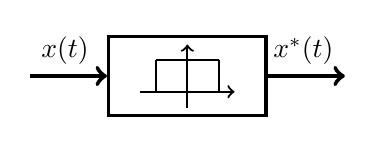
\begin{tikzpicture}[scale=2]
    \node[block](aa)at(3.5,-0.5){};
    \draw[->, thick](3.2,-0.6)--(3.8,-0.6);
    \draw[->, thick](3.5,-0.7)--(3.5,-0.3);
    \draw[-,thick](3.3,-0.4)--(3.7,-0.4);
    \draw[-,thick](3.3,-0.4)--(3.3,-0.6);
    \draw[-,thick](3.7,-0.4)--(3.7,-0.6);
    \draw[->,ultra thick](2.5,-0.5)node[above right]{$x(t)$}--(aa.180);
    \draw[->,ultra thick](aa.0)--(4.5,-0.5)node[above left]{$x^*(t)$};
\end{tikzpicture}
\end{document}